\documentclass[runningheads]{llncs}

\usepackage[T1]{fontenc}
\usepackage{graphicx}
\usepackage{amsmath,amssymb}
\usepackage{algorithm}
\usepackage{algorithmic}
\usepackage{booktabs}
\usepackage{multirow}
\usepackage{xcolor}
\usepackage{hyperref}
\usepackage{cleveref}

% Custom commands
\newcommand{\R}{\mathbb{R}}
\newcommand{\N}{\mathcal{N}}
\newcommand{\E}{\mathbb{E}}
\newcommand{\G}{\mathcal{G}}
\newcommand{\bW}{\mathbf{W}}
\newcommand{\bx}{\mathbf{x}}
\newcommand{\bh}{\mathbf{h}}
% \newcommand{\bhh}{\hat{\mathbf{h}}} % unused

\begin{document}

\title{Cost-Sensitive Neighborhood Aggregation\\for Heterophilous Graphs:\\When Does Per-Edge Routing Help?}

\titlerunning{CSNA: When Does Per-Edge Routing Help?}

\author{Eyal Weiss\orcidID{0000-0003-0508-6213}}

\authorrunning{E. Weiss}

\institute{Computer Science Faculty, Technion --- Israel Institute of Technology\\
\email{eweiss@campus.technion.ac.il}}

\maketitle

\begin{abstract}
Recent work distinguishes two heterophily regimes: \emph{adversarial}, where cross-class edges dilute class signal and harm classification, and \emph{informative}, where the heterophilous structure itself carries useful signal.
We ask: \emph{when does per-edge message routing help, and when is a uniform spectral channel sufficient?}
To operationalize this question we introduce \emph{Cost-Sensitive Neighborhood Aggregation} (CSNA), a GNN layer that computes pairwise distance in a learned projection and uses it to soft-route each message through concordant and discordant channels with independent transformations.
Under a contextual stochastic block model we show that mean aggregation can reverse the label-aligned signal direction under heterophily, and that cost-sensitive weighting with $w_+/w_- > q/p$ preserves the correct sign.
On six benchmarks with uniform tuning, CSNA is competitive with state-of-the-art methods on adversarial-heterophily datasets (Texas, Wisconsin, Cornell, Actor) but underperforms on informative-heterophily datasets (Chameleon, Squirrel)---precisely the regime where per-edge routing has no useful decomposition to exploit.
The pattern is itself the finding: the cost function's ability to separate edge types serves as a diagnostic for the heterophily regime, revealing \emph{when} fine-grained routing adds value over uniform channels and when it does not.
Code is available at \url{https://github.com/eyal-weiss/CSNA-public}.

\keywords{Graph Neural Networks \and Heterophily \and Message Passing \and Cost-Sensitive Aggregation}
\end{abstract}

%% ================================================================
\section{Introduction}\label{sec:intro}
%% ================================================================

Message-passing Graph Neural Networks (GNNs)~\cite{kipf2017semi,velickovic2018graph,hamilton2017inductive} aggregate features from a node's neighborhood under an implicit \emph{homophily} assumption: connected nodes share labels or properties.
When this assumption holds, aggregation smooths representations within a class and yields strong node classification~\cite{wu2020comprehensive}.
However, many real-world graphs exhibit \emph{heterophily}---connected nodes frequently differ in label~\cite{pei2020geom,zhu2020beyond}---and on such graphs standard GNNs can perform worse than a simple Multi-Layer Perceptron (MLP) that ignores graph structure entirely, because aggregation \emph{dilutes} rather than \emph{reinforces} class signal~\cite{zhu2020beyond}.

Several architectures address heterophily: H2GCN~\cite{zhu2020beyond} separates ego from multi-hop neighbor representations; GPRGNN~\cite{chien2021adaptive} learns polynomial graph filter coefficients; ACM-GNN~\cite{luan2022revisiting} mixes low-pass, high-pass, and identity channels with per-node gating.
These methods share a common intuition---that different edges carry different quality of information for classification---but differ in \emph{how} they distinguish edges.
ACM-GNN, the most closely related prior work, uses three fixed spectral channels (aggregation, diversification, identity) that are uniform within each channel: every edge receives the same treatment within a given channel.

We propose \emph{Cost-Sensitive Neighborhood Aggregation} (CSNA), which takes a different approach: compute pairwise distance in a learned projection space, and use this distance to soft-route each message through two channels---concordant (low cost, likely same-class) and discordant (high cost, likely different-class)---each with its own learned transformation.
A per-node gating mechanism then combines the channels with an ego (the node's own) representation.
The key difference from ACM-GNN is that CSNA's routing is \emph{per-edge}: each edge receives an individualized routing weight based on the learned distance between its endpoints, rather than a uniform spectral filter applied identically to all edges.
This finer granularity comes at the cost of additional per-edge computation (3--10$\times$ overhead vs.\ GCN; see \Cref{app:runtime}).

\paragraph{Contributions.}
(1)~We characterize when per-edge routing helps: CSNA's learned cost function achieves strong edge-type separation on adversarial-heterophily datasets but not on informative-heterophily datasets, operationalizing the regime distinction through a concrete diagnostic (\Cref{sec:experiments}).
(2)~We introduce CSNA, a dual-channel message-passing layer with per-edge cost-based routing (\Cref{sec:method}); the default (``lite'') version uses only observed divergence $g_{ij}$ in a learned projection; an extended version adds a learned component $h_{ij}$.
(3)~Under a contextual stochastic block model (CSBM), we prove that mean aggregation can reverse the label-aligned signal direction under heterophily, and that cost-sensitive weighting with $w_+/w_- > q/p$ preserves the correct sign (\Cref{sec:theory}).


%% ================================================================
\section{Related Work}\label{sec:related}
%% ================================================================

\paragraph{Heterophily-aware GNNs.}
Standard GNNs (GCN~\cite{kipf2017semi}, GAT~\cite{velickovic2018graph}, GraphSAGE~\cite{hamilton2017inductive}) degrade as homophily decreases~\cite{zhu2020beyond}.
H2GCN~\cite{zhu2020beyond} separates ego from higher-order neighbor embeddings.
GPRGNN~\cite{chien2021adaptive} learns polynomial graph filter coefficients that can model both low-pass and high-pass responses.
FAGCN~\cite{bo2021beyond} assigns positive or negative attention weights.
ACM-GNN~\cite{luan2022revisiting} is the most closely related method: it decomposes aggregation into three spectral channels (low-pass, high-pass, identity) and combines them with per-node gating.
CSNA shares the dual-channel-plus-gating architecture but replaces uniform spectral filters with per-edge learned routing.

\paragraph{Distinction from ACM-GNN.}
Both ACM-GNN and CSNA route messages through multiple channels and gate the output per-node.
The difference is in channel construction: ACM-GNN's channels are defined by fixed spectral operations (mean aggregation for low-pass, signed aggregation for high-pass), so every edge within a channel is treated identically.
CSNA computes a per-edge concordance score from learned pairwise distance and uses it to route each edge independently.
This is finer-grained but more expensive: ACM-GNN has the same asymptotic cost as GCN ($O(|E| \cdot d)$ per channel, but with fixed structure), while CSNA requires an additional $O(|E| \cdot d)$ distance computation.

\paragraph{When per-edge routing helps: a toy example.}
\Cref{fig:toy} illustrates the key scenario where per-edge routing outperforms uniform spectral channels.
Consider a heterophilous graph in which most edges are cross-class, but the cross-class edges have \emph{mixed utility}: some neighbors' features, when transformed, carry complementary information that aids classification, while others are misleading.
A uniform high-pass channel (as in ACM-GNN) treats all cross-class edges identically---it cannot distinguish helpful from harmful heterophilous neighbors.
CSNA's per-edge cost function assigns an individual routing weight to each edge, so the model can upweight informative cross-class edges and downweight misleading ones.
This advantage materializes when node features within a class are not homogeneous---some cross-class neighbors provide complementary signal while others contribute noise---precisely the adversarial-heterophily regime.
On informative-heterophily datasets, where nearly all heterophilous edges carry useful structural signal, the per-edge decomposition has no useful separation to exploit and the extra routing overhead buys nothing.

\begin{figure}[t]
\centering
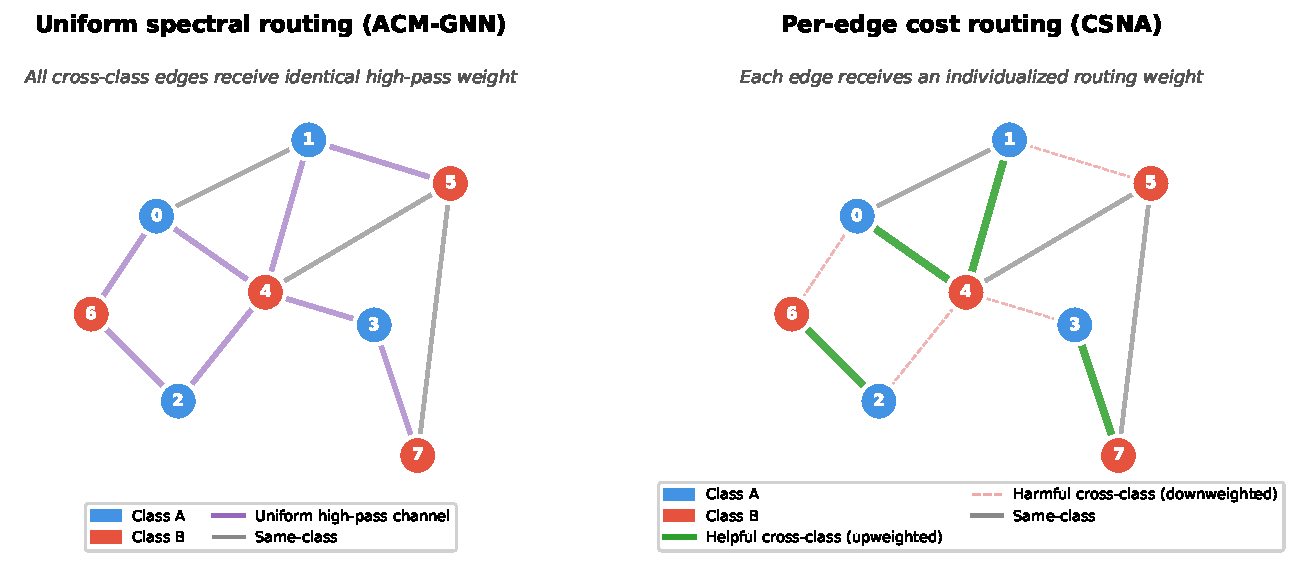
\includegraphics[width=0.95\textwidth]{figures/toy_example.pdf}
\vspace{-2mm}
\caption{Toy example: a heterophilous graph where cross-class edges have mixed utility. \textbf{Left:} ACM-GNN's uniform high-pass channel assigns identical weight to all cross-class edges. \textbf{Right:} CSNA's per-edge cost routing upweights helpful cross-class edges (thick green) and downweights harmful ones (thin dashed red). This distinction is possible only when the cost function can separate edge types---the adversarial-heterophily regime.}\label{fig:toy}
\end{figure}

\paragraph{Over-smoothing and over-squashing.}
These pathologies~\cite{li2018deeper,oono2020graph,alon2021on,topping2022understanding} are compounded under heterophily.
Cost-based routing reduces cross-class smoothing but does not address over-squashing, which is a topological bottleneck issue.


%% ================================================================
\section{Method}\label{sec:method}
%% ================================================================

\subsection{Preliminaries}

Let $\G = (V, E)$ be an undirected graph with $n = |V|$ nodes and feature matrix $\mathbf{X} \in \R^{n \times d}$.
Each node $i$ has a label $y_i \in \{1, \ldots, C\}$.
The \emph{edge homophily ratio} is $\mathcal{H} = |\{(i,j) \in E : y_i = y_j\}|/|E|$.

In standard message-passing~\cite{gilmer2017neural}, node $i$'s representation at layer $\ell+1$ is:
\begin{equation}\label{eq:mp}
    \bh_i^{(\ell+1)} = \sigma\!\Bigl(\sum_{j \in \N(i)} \alpha_{ij}\, \bW^{(\ell)}\, \bh_j^{(\ell)}\Bigr),
\end{equation}
where $\N(i)$ includes $i$ itself, $\alpha_{ij}$ are aggregation weights, and $\sigma$ is a nonlinearity.

\subsection{Cost-Sensitive Neighborhood Aggregation}\label{sec:csna}

The core idea is simple: compute pairwise distance in a learned projection, use it to soft-route messages through two channels.

\paragraph{Step 1: Edge cost (observed divergence).}
For each edge $(i,j)$ at layer $\ell$, we compute a distance in a learned projection:
\begin{equation}\label{eq:g}
    g_{ij}^{(\ell)} = \|\bW_g\, \bh_i^{(\ell)} - \bW_g\, \bh_j^{(\ell)}\|_2,
\end{equation}
where $\bW_g \in \R^{d' \times d}$ is a learned projection matrix.
Low $g_{ij}$ indicates the endpoints are similar in the projected space (likely concordant); high $g_{ij}$ indicates divergence (likely discordant).
This is the only cost component in the default (lite) version of CSNA.

\paragraph{Step 2: Concordance routing.}
The cost is converted to a soft concordance score:
\begin{equation}\label{eq:concordance}
    s_{ij}^{(\ell)} = \sigma\!\left(\frac{-g_{ij}^{(\ell)}}{\tau}\right) \in (0, 1),
\end{equation}
where $\tau > 0$ is a temperature parameter and $\sigma$ is the sigmoid function.
High concordance (low cost) routes the message toward the concordant channel; low concordance (high cost) routes it toward the discordant channel.

\paragraph{Step 3: Dual-channel aggregation.}
Messages are routed through two channels with independent transformations:
\begin{align}
    \bh_i^{\text{con}} &= \sum_{j \in \N(i)} \tilde{s}_{ij}\, \bW_{\text{con}}\, \bh_j^{(\ell)}, \label{eq:con}\\
    \bh_i^{\text{dis}} &= \sum_{j \in \N(i)} \tilde{d}_{ij}\, \bW_{\text{dis}}\, \bh_j^{(\ell)}, \label{eq:dis}
\end{align}
where $\tilde{s}_{ij} = \mathrm{softmax}_{j \in \N(i)}(s_{ij})$, $\tilde{d}_{ij} = \mathrm{softmax}_{j \in \N(i)}(1 - s_{ij})$, and $\bW_{\text{con}}, \bW_{\text{dis}} \in \R^{d' \times d}$ are independent weight matrices.
The concordant channel emphasizes likely same-class neighbors; the discordant channel processes likely different-class neighbors through a separate transformation.

\paragraph{Step 4: Gated combination.}
The final output combines both channels with the ego representation via per-node gating:
\begin{equation}\label{eq:gate}
    \bh_i^{(\ell+1)} = \sum_{k \in \{\text{con}, \text{dis}, \text{self}\}} \gamma_k(\bh_i) \cdot \bh_i^{k},
\end{equation}
where $\bh_i^{\text{self}} = \bW_{\text{self}}\, \bh_i^{(\ell)}$ and $\gamma(\bh_i) = \mathrm{softmax}(\bW_\gamma [\bh_i^{\text{con}} \| \bh_i^{\text{dis}} \| \bh_i^{\text{self}}]) \in \R^3$.

\paragraph{Extended variant: $g + h$.}
An optional extension adds a learned cost component:
\begin{equation}\label{eq:f}
    f_{ij}^{(\ell)} = g_{ij}^{(\ell)} + h_{ij}^{(\ell)}, \quad\text{where}\quad h_{ij}^{(\ell)} = \mathrm{softplus}\bigl(\mathbf{a}^\top [\bW_g \bh_i^{(\ell)} \| \bW_g \bh_j^{(\ell)}]\bigr),
\end{equation}
where $[\cdot \| \cdot]$ denotes vector concatenation, $\mathbf{a} \in \R^{2d'}$ is a learnable parameter vector, and $f_{ij}$ replaces $g_{ij}$ in \Cref{eq:concordance}.
In our experiments, the extended variant wins clearly only on Wisconsin (84.1 vs.\ 79.6); on all other datasets the lite version performs comparably or better (\Cref{app:variants}).
We therefore present the lite version ($g_{ij}$ only) as the default.

\paragraph{Calibration regularization.}
When training with labels, we add a regularizer that penalizes cost overestimation on same-class edges:
\begin{equation}\label{eq:cal}
    \mathcal{L}_{\text{cal}} = \frac{1}{|E_{\text{train}}|} \sum_{(i,j) \in E_{\text{train}}} \bigl[\mathrm{ReLU}(g_{ij} - \mathbb{1}[y_i \neq y_j])\bigr]^2,
\end{equation}
where $E_{\text{train}}$ denotes edges between labeled nodes.
The full objective is $\mathcal{L} = \mathcal{L}_{\text{CE}} + \lambda_{\text{cal}}\, \mathcal{L}_{\text{cal}}$, with $\lambda_{\text{cal}} = 0.1$ fixed across all experiments.
Note that $g_{ij}$ and the binary indicator $\mathbb{1}[y_i \neq y_j]$ are on different scales; the regularizer acts as a soft penalty that directly shapes the routing signal, encouraging lower costs (and thus higher concordance) for same-class edges.

\paragraph{Architecture details.}
We apply an input MLP before the first CSNA layer, add residual connections, and initialize the gate bias to $[0, 0, 1]$ (favoring the ego channel so the model starts near MLP-like behavior).
Self-loops are added before cost computation; they receive $g_{ii}=0$, so ego information flows primarily through the concordant and self channels.
The softmax normalization of concordance weights is performed per source node; we also tested per-destination normalization (more common in message-passing GNNs) and found no consistent difference across datasets.

The CSNA layer is summarized in Algorithm~\ref{alg:csna}.

\begin{algorithm}[t]
\caption{CSNA Layer (Lite Version)}\label{alg:csna}
\begin{algorithmic}[1]
\REQUIRE Node features $\mathbf{H}^{(\ell)} \in \R^{n \times d}$, edge index $E$, temperature $\tau$
\ENSURE Updated features $\mathbf{H}^{(\ell+1)} \in \R^{n \times d'}$
\FOR{each edge $(i,j) \in E$}
    \STATE $g_{ij} \leftarrow \|\bW_g \bh_i - \bW_g \bh_j\|_2$ \COMMENT{Pairwise distance in learned projection}
    \STATE $s_{ij} \leftarrow \sigma(-g_{ij}/\tau)$ \COMMENT{Concordance score}
\ENDFOR
\FOR{each node $i \in V$}
    \STATE $\bh_i^{\text{con}} \leftarrow \sum_{j \in \N(i)} \tilde{s}_{ij}\, \bW_{\text{con}} \bh_j$ \COMMENT{Concordant channel}
    \STATE $\bh_i^{\text{dis}} \leftarrow \sum_{j \in \N(i)} \tilde{d}_{ij}\, \bW_{\text{dis}} \bh_j$ \COMMENT{Discordant channel}
    \STATE $\bh_i^{\text{self}} \leftarrow \bW_{\text{self}} \bh_i$ \COMMENT{Ego transform}
    \STATE $\bh_i^{(\ell+1)} \leftarrow \sum_k \gamma_k(\bh_i) \cdot \bh_i^k$ \COMMENT{Gated combination}
\ENDFOR
\end{algorithmic}
\end{algorithm}


%% ================================================================
\section{Theoretical Analysis}\label{sec:theory}
%% ================================================================

We analyze the advantage of cost-sensitive aggregation over mean aggregation in heterophilous settings using the \emph{contextual stochastic block model} (CSBM)~\cite{zhu2020beyond}.
Our analysis uses the binary ($C=2$) case for tractability; our experimental datasets have $C=5$, and we discuss the multi-class extension in \Cref{app:multiclass}.
Importantly, the theorems below apply to \emph{any} weighted aggregation scheme---they are not specific to the $g+h$ decomposition or the lite variant.

\begin{definition}[Contextual Stochastic Block Model]\label{def:csbm}
A graph $\G$ is drawn from $\mathrm{CSBM}(n, 2, p, q, \mu)$ with $n$ nodes in two equal-sized classes $V_+, V_-$.
Edges are drawn independently: probability $p$ within classes, probability $q$ between classes.
Node features: $\bx_i \sim \mathcal{N}(\boldsymbol{\mu}_{y_i}, \mathbf{I}_d)$, with $\boldsymbol{\mu}_+ = +\frac{\mu}{2}\mathbf{e}_1$ and $\boldsymbol{\mu}_- = -\frac{\mu}{2}\mathbf{e}_1$.
\end{definition}

The homophily ratio is $\mathcal{H} = p/(p + q)$.
The heterophilous regime is $q > p$, i.e., $\mathcal{H} < 1/2$.

\begin{theorem}[Signal distortion under mean aggregation]\label{thm:degradation}

\noindent Let $\G \sim \mathrm{CSBM}(n, 2, p, q, \mu)$ with constant $p, q \in (0,1)$ and equal class sizes.
After one round of symmetrically normalized aggregation with self-loops, $\mathbf{H}^{(1)} = \tilde{\mathbf{A}} \mathbf{X}$, where $\tilde{\mathbf{A}} = \mathbf{D}^{-1/2}(\mathbf{A}+\mathbf{I})\mathbf{D}^{-1/2}$, the expected class-mean representations satisfy:
\begin{equation}
    \E[\bar{\bh}_+^{(1)} - \bar{\bh}_-^{(1)}] = \frac{p-q}{p+q}(\boldsymbol{\mu}_+ - \boldsymbol{\mu}_-) + O(1/n),
\end{equation}
where $\bar{\bh}_c^{(1)}$ is the mean representation of class $c$.
The scaling factor $\lambda = (p-q)/(p+q)$ is signed: when $q > p$, it is negative, reversing the label-aligned signal direction.
The magnitude $|\lambda|$ is attenuated (strictly less than $1$) whenever $q \neq p$, and is minimized near $p = q$.
In the extreme heterophily limit $q \gg p$, $|\lambda|$ approaches $1$---strong heterophily distorts but does not collapse the signal.
\end{theorem}

\begin{proof}
Under the dense CSBM, $d_i = \Theta(n)$, so the self-loop in $\mathbf{A}+\mathbf{I}$ contributes $O(1/n)$ per node and does not affect the leading coefficient.
For a node $i \in V_+$, same-class neighbors number $n_s(i) \sim \mathrm{Bin}(n/2-1, p)$ and different-class neighbors $n_d(i) \sim \mathrm{Bin}(n/2, q)$.
At leading order:
\begin{align}
    \E[\bh_i^{(1)} | y_i = +1] &= \frac{p}{p+q}\boldsymbol{\mu}_+ + \frac{q}{p+q}\boldsymbol{\mu}_- + O(1/n) = \frac{p-q}{p+q} \cdot \frac{\mu}{2}\mathbf{e}_1 + O(1/n),
\end{align}
where the $O(1/n)$ term absorbs both the self-loop contribution and the concentration error (by Hoeffding's inequality, $n_s(i)/d_i$ concentrates around $p/(p+q)$ at rate $O(1/\sqrt{n})$, giving $O(1/n)$ after averaging over $n/2$ nodes per class).
By symmetry and averaging: $\E[\bar{\bh}_+^{(1)} - \bar{\bh}_-^{(1)}] = \frac{p-q}{p+q}(\boldsymbol{\mu}_+ - \boldsymbol{\mu}_-) + O(1/n)$. \qed
\end{proof}

\begin{theorem}[Cost-sensitive aggregation preserves signal direction]\label{thm:preservation}
Under the same CSBM, suppose an aggregation scheme weights each edge $(i,j)$ by $w_{ij}$, with $\E[w_{ij} | y_i = y_j] = w_+$ and $\E[w_{ij} | y_i \neq y_j] = w_-$, where $w_+ > w_- \geq 0$.
Then:
\begin{equation}
    \E[\bar{\bh}_+^{(1)} - \bar{\bh}_-^{(1)}] = \frac{p\,w_+ - q\,w_-}{p\,w_+ + q\,w_-}(\boldsymbol{\mu}_+ - \boldsymbol{\mu}_-) + O(1/n).
\end{equation}
The scaling factor is positive---preserving the original class direction---if and only if $w_+/w_- > q/p$.
\end{theorem}

\begin{proof}
Replacing uniform weights with $w_+$ and $w_-$ in the proof of \Cref{thm:degradation}:
\begin{align}
    \E[\bh_i^{(1)} | y_i = +1] &= \frac{p\, w_+}{p\, w_+ + q\, w_-}\boldsymbol{\mu}_+ + \frac{q\, w_-}{p\, w_+ + q\, w_-}\boldsymbol{\mu}_- + O(1/n).
\end{align}
Setting $w_+=w_-=1$ recovers \Cref{thm:degradation}.
The numerator $p\,w_+ - q\,w_- > 0$ iff $w_+/w_- > q/p$. \qed
\end{proof}

\begin{remark}[Applicability to CSNA]
\Cref{thm:preservation} applies to CSNA's concordant channel with $w_{ij} = s_{ij}$.
The condition $s_+/s_- > q/p$ requires the cost function to assign sufficiently higher concordance to same-class edges; the calibration regularizer (\Cref{eq:cal}) encourages this.
\Cref{thm:preservation} is \emph{conditional}: it shows what happens \emph{if} the cost function achieves the separation, not that CSNA \emph{will} learn it.
\end{remark}

\begin{remark}[Scope and limitations]\label{rem:scope}
(i)~The CSBM analysis is for $C=2$; experiments have $C=5$.
The qualitative conclusion carries over (\Cref{app:multiclass}), but the quantitative bound changes.
(ii)~\Cref{thm:preservation} bounds the class-mean difference, not classification accuracy: a sign-reversed but well-separated representation can be corrected by a downstream linear classifier.
The theorems show that cost-sensitive weighting \emph{preserves the label-aligned signal direction} where mean aggregation may reverse it; they do not prove improved classification in isolation.
(iii)~The analysis covers a single layer; multi-layer interactions between evolving representations and the cost function are not analyzed.
\end{remark}


%% ================================================================
\section{Experiments}\label{sec:experiments}
%% ================================================================

\subsection{Datasets}

We evaluate on six heterophily benchmarks (Table~\ref{tab:datasets}).
Texas, Wisconsin, and Cornell are webpage graphs from WebKB~\cite{pei2020geom}.
Chameleon and Squirrel are Wikipedia article networks~\cite{pei2020geom}.
Actor is a co-occurrence network from film databases~\cite{pei2020geom}.
We note that Chameleon and Squirrel have known data quality issues (duplicate nodes)~\cite{platonov2023critical}.

\begin{table}[t]
\caption{Dataset statistics. $\mathcal{H}$ is the edge homophily ratio.}\label{tab:datasets}
\centering
\begin{tabular}{lccccc}
\toprule
Dataset & Nodes & Edges & Features & Classes & $\mathcal{H}$ \\
\midrule
Texas & 183 & 287 & 1,703 & 5 & 0.09 \\
Wisconsin & 251 & 458 & 1,703 & 5 & 0.19 \\
Cornell & 183 & 278 & 1,703 & 5 & 0.13 \\
Actor & 7,600 & 26,705 & 932 & 5 & 0.22 \\
Chameleon & 2,277 & 31,396 & 2,325 & 5 & 0.23 \\
Squirrel & 5,201 & 198,423 & 2,089 & 5 & 0.22 \\
\bottomrule
\end{tabular}
\end{table}

\subsection{Setup}

\paragraph{Baselines.}
We compare against: (1)~\textbf{MLP} (no graph structure), (2)~\textbf{GCN}~\cite{kipf2017semi}, (3)~\textbf{GAT}~\cite{velickovic2018graph}, (4)~\textbf{GraphSAGE}~\cite{hamilton2017inductive}, (5)~\textbf{H2GCN}~\cite{zhu2020beyond}, (6)~\textbf{GPRGNN}~\cite{chien2021adaptive}, and (7)~\textbf{ACM-GNN}~\cite{luan2022revisiting}.

\paragraph{Protocol.}
We use 10 random 60\%/20\%/20\% splits (seed 42).
\emph{All methods} are tuned over the same hyperparameter grid: learning rate $\in \{0.01, 0.005\}$, hidden dimension $\in \{64, 128\}$ on small datasets (Texas, Wisconsin, Cornell) and $\{64\}$ on large datasets (Actor, Chameleon, Squirrel) for computational efficiency.
CSNA additionally tunes temperature $\tau \in \{0.1, 0.5, 1.0, 2.0\}$.
Tuning uses 3 validation splits on small datasets and 2 on large datasets.
All models use 2 layers, dropout 0.5, Adam with weight decay $5 \times 10^{-4}$, and early stopping (patience 50, max 300 epochs).
We save the checkpoint with best validation accuracy and evaluate it \emph{once} on test.
We report classification accuracy (fraction of correctly labeled test nodes), averaged over 10 splits, with standard deviation reflecting split-to-split variability.
CSNA here is the lite version ($g_{ij}$ only, no sampling).
Complete details in \Cref{app:repro}.

\subsection{Main Results}

Results are in Table~\ref{tab:results}.

\begin{table}[t]
\caption{Node classification accuracy (\%) on heterophily benchmarks. All methods tuned over the same grid. Best in \textbf{bold}, second-best \underline{underlined}.}\label{tab:results}
\centering
\setlength{\tabcolsep}{3.5pt}
\small
\begin{tabular}{lcccccc}
\toprule
Method & Texas & Wisconsin & Cornell & Actor & Chameleon & Squirrel \\
 & $\mathcal{H}$=0.09 & $\mathcal{H}$=0.19 & $\mathcal{H}$=0.13 & $\mathcal{H}$=0.22 & $\mathcal{H}$=0.23 & $\mathcal{H}$=0.22 \\
\midrule
MLP & 77.3{\tiny$\pm$4.6} & \textbf{83.7{\tiny$\pm$4.8}} & \underline{72.2{\tiny$\pm$3.6}} & 35.0{\tiny$\pm$1.4} & 51.9{\tiny$\pm$1.8} & 34.8{\tiny$\pm$1.4} \\
GCN & 55.7{\tiny$\pm$9.9} & 50.6{\tiny$\pm$8.5} & 47.0{\tiny$\pm$8.7} & 27.3{\tiny$\pm$1.4} & \textbf{67.3{\tiny$\pm$1.7}} & \textbf{53.4{\tiny$\pm$0.8}} \\
GAT & 50.8{\tiny$\pm$9.8} & 51.4{\tiny$\pm$7.8} & 47.3{\tiny$\pm$5.8} & 28.0{\tiny$\pm$1.4} & 65.7{\tiny$\pm$2.2} & 50.4{\tiny$\pm$1.4} \\
GraphSAGE & 76.5{\tiny$\pm$6.8} & 75.9{\tiny$\pm$5.8} & 66.2{\tiny$\pm$7.7} & 34.1{\tiny$\pm$0.6} & 63.9{\tiny$\pm$2.1} & 45.8{\tiny$\pm$1.4} \\
H2GCN & \textbf{81.9{\tiny$\pm$4.2}} & \underline{82.4{\tiny$\pm$5.8}} & \underline{72.2{\tiny$\pm$4.2}} & 35.6{\tiny$\pm$0.9} & 56.8{\tiny$\pm$2.7} & 35.0{\tiny$\pm$1.3} \\
GPRGNN & \underline{77.8{\tiny$\pm$6.9}} & 75.7{\tiny$\pm$7.7} & 58.6{\tiny$\pm$9.9} & \textbf{36.0{\tiny$\pm$0.8}} & 65.0{\tiny$\pm$2.1} & 43.6{\tiny$\pm$1.8} \\
ACM-GNN & 77.3{\tiny$\pm$8.2} & 78.0{\tiny$\pm$4.4} & 68.6{\tiny$\pm$7.2} & 35.3{\tiny$\pm$1.2} & \underline{65.9{\tiny$\pm$2.9}} & \underline{51.0{\tiny$\pm$1.8}} \\
\midrule
CSNA (ours) & 77.0{\tiny$\pm$8.3} & 79.6{\tiny$\pm$6.2} & \textbf{72.7{\tiny$\pm$4.3}} & \underline{35.7{\tiny$\pm$1.2}} & 54.6{\tiny$\pm$2.7} & 37.8{\tiny$\pm$1.9} \\
\bottomrule
\end{tabular}
\end{table}

The results reveal a clear split between two types of heterophily benchmarks.
Note that many differences across methods are within one standard deviation; we focus on patterns rather than strict mean rankings.

\textbf{Adversarial heterophily (Texas, Wisconsin, Cornell, Actor).}
On these datasets, cross-class edges are adversarial: aggregating neighbor features degrades classification.
MLP is a strong baseline, and standard GNNs (GCN, GAT) perform poorly.
H2GCN is the strongest method on Texas (81.9) and Wisconsin (82.4), where its ego-separated multi-hop design is effective.
CSNA is competitive: it is statistically tied for first on Cornell (72.7 vs.\ H2GCN 72.2 and MLP 72.2, all within $\sim$0.5pp) and on Actor (35.7 vs.\ GPRGNN 36.0 and H2GCN 35.6, all within $\sim$0.4pp---well within one standard deviation).
On Texas and Wisconsin, CSNA trails H2GCN but remains within one standard deviation of the other heterophily-aware methods.

\textbf{Informative heterophily (Chameleon, Squirrel).}
On these datasets, heterophilous structure itself carries useful signal.
GCN remains the top performer (67.3 on Chameleon, 53.4 on Squirrel), but ACM-GNN is close on both datasets (65.9 and 51.0, within 1--2pp of GCN), while CSNA (54.6 and 37.8) and H2GCN (56.8 and 35.0) trail substantially.
CSNA's cost-based routing cannot distinguish ``harmful'' from ``useful'' heterophilous edges---methods that apply uniform spectral filters (ACM-GNN, GPRGNN) or standard aggregation (GCN) handle this regime better.
This distinction---between adversarial and informative heterophily---is increasingly recognized~\cite{luan2022revisiting,platonov2023critical} and suggests that no single approach dominates all heterophily regimes.
CSNA's cost semantics make the distinction explicit: on adversarial datasets, learned costs successfully separate edge types (Fig.~\ref{fig:cost_dist}); on informative datasets, they cannot.

\begin{figure}[t]
\centering
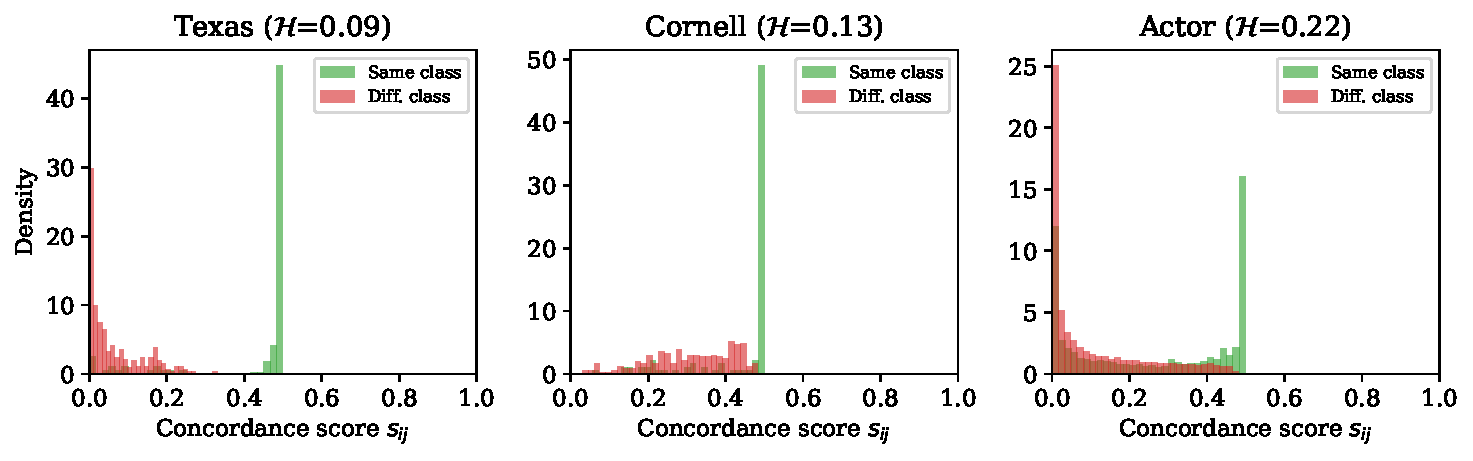
\includegraphics[width=0.9\textwidth]{figures/cost_distribution.pdf}
\vspace{-2mm}
\caption{Learned concordance scores $s_{ij}$ for same-class (green) and different-class (red) edges on three datasets. On adversarial-heterophily datasets (Texas, Cornell), the distributions are well separated; on Actor, overlap is larger. Generated using the extended ($g+h$) variant; similar separation is observed with the lite version.}\label{fig:cost_dist}
\end{figure}

\paragraph{Comparison with ACM-GNN.}
ACM-GNN and CSNA share the dual-channel-plus-gating architecture but differ in routing granularity.
On adversarial-heterophily datasets, their accuracy is comparable: CSNA leads on Cornell (+4.1pp) and Actor (+0.4pp), while ACM-GNN edges ahead on Wisconsin.
The clearest separation appears on informative-heterophily datasets, where ACM-GNN's uniform spectral channels are substantially more effective: ACM-GNN outperforms CSNA by 11.3pp on Chameleon and 13.2pp on Squirrel.
This suggests that when heterophilous edges carry uniformly useful signal, fixed spectral filters preserve it better than per-edge routing, which may over-differentiate edges that are equally informative.
\paragraph{Routing quality as a diagnostic.}
To quantify the cost function's ability to discriminate edge types, we compute the AUC of the concordance score $s_{ij}$ as a binary classifier for same-class vs.\ different-class edges.
On the adversarial-heterophily datasets, AUC ranges from 0.48 (Texas) to 0.83 (Wisconsin), while on informative-heterophily datasets it is 0.55--0.57 (Chameleon, Squirrel).
Interestingly, CSNA's accuracy gain over GCN does not correlate simply with AUC: Texas has near-random AUC (0.48) yet CSNA outperforms GCN by 21pp, while Wisconsin has the highest AUC (0.83) and the largest gain (+29pp).
This suggests that CSNA's benefit comes not only from edge-type separation but also from the dual-channel architecture and gating mechanism, which can learn useful representations even when the cost function's discrimination is weak.
On informative-heterophily datasets, both the low AUC and the poor accuracy confirm that the cost function cannot usefully decompose the neighborhood.

\paragraph{Ablation highlights.}
We tested four CSNA variants in a factorial design (\Cref{app:variants}): the extended model ($g+h$) vs.\ the lite default ($g$ only), each with and without stochastic edge sampling~\cite{rong2020dropedge}.
The extended variant wins clearly only on Wisconsin (84.1 vs.\ 79.6); on all other datasets the lite version matches or exceeds it.
Edge sampling slightly reduces accuracy (1--3pp) but provides regularization and scaling benefits.
These results motivate presenting the lite version without sampling as the default.


%% ================================================================
\section{Discussion}\label{sec:discussion}
%% ================================================================

\paragraph{Limitations---and what they reveal.}
\begin{itemize}
    \item \textbf{Homophilous graphs.} CSNA underperforms GCN by 4--11pp on Cora, CiteSeer, and PubMed (\Cref{app:homophily}). The per-edge routing is not justified when standard aggregation suffices; this is expected, since the cost function has little to separate when most edges are already same-class.
    \item \textbf{Informative heterophily.} CSNA underperforms GCN on Chameleon (by 12.7pp) and Squirrel (by 15.6pp), and trails ACM-GNN by 11--13pp on both. Rather than a mere negative result, this failure is diagnostic: it identifies datasets where heterophilous edges are uniformly informative and per-edge routing over-differentiates edges that carry equally useful signal. Fixed spectral filters (ACM-GNN) and standard aggregation (GCN) better preserve this signal.
    \item \textbf{Computational cost.} CSNA is 3--10$\times$ slower than GCN (\Cref{app:runtime}), though it uses fewer parameters.
    \item \textbf{Comparison with ACM-GNN.} CSNA shares the dual-channel-plus-gating design with ACM-GNN~\cite{luan2022revisiting}. On adversarial-heterophily datasets the methods achieve comparable accuracy; on informative-heterophily datasets ACM-GNN is clearly superior. The per-edge routing is a meaningful architectural difference whose value is regime-dependent.
\end{itemize}


%% ================================================================
\section{Conclusion}\label{sec:conclusion}
%% ================================================================

We presented CSNA, a GNN layer that computes pairwise distance in a learned projection and uses it to soft-route messages through concordant and discordant channels, with per-node gating.
The key architectural difference from the closely related ACM-GNN is per-edge routing rather than uniform spectral channels---a finer-grained mechanism that is competitive on adversarial-heterophily datasets but underperforms on informative-heterophily datasets where uniform filters are more effective.
Our theoretical analysis provides a clean condition ($w_+/w_- > q/p$) under which cost-sensitive weighting preserves the label-aligned signal direction that mean aggregation may reverse.
The results operationalize the adversarial/informative heterophily distinction: CSNA's cost function achieves meaningful edge-type separation only in the adversarial regime, serving as a diagnostic for the nature of heterophily in a given graph.
The clearest open question is whether per-edge routing can be adapted to the informative-heterophily regime---possibly by learning to leverage rather than suppress cross-class signal.


%% ================================================================
\bibliographystyle{splncs04}
\bibliography{references}

%% ================================================================
\appendix
\section*{Appendix}
\addcontentsline{toc}{section}{Appendix}

\section{CSNA Variant Comparison}\label{app:variants}

We compare four CSNA variants in a factorial design: full ($g+h$) vs.\ lite ($g$ only) $\times$ edge sampling vs.\ no sampling.
Results are in Table~\ref{tab:variants}.

\begin{table}[h]
\caption{CSNA variant comparison: accuracy (\%) on all six datasets. ``Full'' includes both $g_{ij}$ and $h_{ij}$; ``lite'' uses $g_{ij}$ only. ``Samp'' applies edge sampling during training.}\label{tab:variants}
\centering
\small
\begin{tabular}{lcccccc}
\toprule
Variant & Texas & Wisconsin & Cornell & Actor & Chameleon & Squirrel \\
\midrule
Full, no samp & 77.0 & \textbf{84.1} & 70.8 & 35.6 & 53.0 & 38.2 \\
Full + samp & 74.1 & 79.8 & 70.5 & \textbf{36.3} & 51.8 & 37.4 \\
Lite, no samp & \textbf{77.0} & 79.6 & \textbf{72.7} & 35.7 & \textbf{54.6} & \textbf{37.8} \\
Lite + samp & 75.7 & 79.6 & 70.3 & 35.8 & 53.5 & 37.0 \\
\bottomrule
\end{tabular}
\end{table}

\paragraph{Discussion.}
The full variant ($g+h$) wins clearly only on Wisconsin (84.1 vs.\ 79.6), where the learned component $h_{ij}$ provides a useful correction beyond observed divergence.
On all other datasets, the lite version matches or exceeds the full version, suggesting that feature divergence $g_{ij}$ alone is a sufficient routing signal.
Since $h_{ij}$ introduces additional learnable parameters without a clear consistent advantage, it risks overfitting---particularly on the small datasets in our benchmark suite.
We therefore use the lite version ($g_{ij}$ only) as the default.

Edge sampling slightly hurts accuracy on most datasets (1--3pp) but may act as a regularizer on Actor (36.3 vs.\ 35.6 for the full variant).
The accuracy cost of sampling is modest, making it a viable strategy for scaling to larger graphs.


\section{Homophily Benchmarks}\label{app:homophily}

To understand CSNA's behavior across the homophily spectrum, we evaluate on three standard homophilous datasets (Table~\ref{tab:homophily}).

\begin{table}[h]
\caption{Accuracy (\%) on homophilous benchmarks. CSNA underperforms GCN by 4--11pp.}\label{tab:homophily}
\centering
\begin{tabular}{lccc}
\toprule
Method & Cora & CiteSeer & PubMed \\
\midrule
GCN & \textbf{77.9} & \textbf{65.7} & \textbf{76.0} \\
CSNA & 67.0 & 56.3 & 72.2 \\
\bottomrule
\end{tabular}
\end{table}

CSNA underperforms GCN by 10.9pp on Cora, 9.4pp on CiteSeer, and 3.8pp on PubMed.
This is expected: on homophilous graphs, standard aggregation is already effective, and the per-edge routing overhead adds complexity without benefit.
The cost function cannot improve on uniform aggregation when most edges are already same-class.
These results suggest CSNA's per-edge routing overhead is not justified on homophilous graphs, where standard aggregation already performs well.


\section{Gate Weight Analysis}\label{app:gate}

Table~\ref{tab:gate_weights} shows the average gate weights at layer 0, revealing dataset-dependent routing strategies.

\begin{table}[h]
\caption{Average gate weights $\gamma$ across nodes (layer 0).}\label{tab:gate_weights}
\centering
\small
\begin{tabular}{lccc}
\toprule
Dataset & $\gamma_{\text{con}}$ & $\gamma_{\text{dis}}$ & $\gamma_{\text{self}}$ \\
\midrule
Texas & 0.30 & 0.13 & 0.57 \\
Wisconsin & 0.00 & 0.00 & 1.00 \\
Cornell & 0.12 & 0.28 & 0.60 \\
Actor & 0.00 & 0.00 & 1.00 \\
Chameleon & 0.34 & 0.66 & 0.00 \\
Squirrel & 0.14 & 0.86 & 0.00 \\
\bottomrule
\end{tabular}
\end{table}

The gate weights reveal three distinct strategies:
\begin{itemize}
    \item \textbf{Self-dominant (Wisconsin, Actor):} The model ignores graph structure entirely ($\gamma_{\text{self}} = 1.0$), effectively reducing to MLP. This is consistent with CSNA matching MLP-level accuracy on these datasets.
    The collapse to MLP-like behavior is itself informative: it indicates that on these datasets, the cost function does not find a useful decomposition of the neighborhood, and the gating mechanism correctly learns to ignore the graph channels.
    \item \textbf{Mixed (Texas, Cornell):} The model uses a combination of ego and graph channels. On Cornell, the discordant channel receives substantial weight ($\gamma_{\text{dis}} = 0.28$), indicating that different-class neighbor information is actively processed.
    \item \textbf{Graph-dominant (Chameleon, Squirrel):} The model relies entirely on graph channels, with the discordant channel dominant ($\gamma_{\text{dis}} = 0.66$ and $0.86$ respectively). Ironically, these are the datasets where CSNA underperforms GCN, suggesting the discordant channel's separate transformation does not capture the useful heterophilous signal as effectively as GCN's uniform aggregation.
\end{itemize}


\section{Runtime and Parameter Comparison}\label{app:runtime}

\begin{table}[h]
\caption{Training time (seconds per split) and parameter count. All on 8-core CPU.}\label{tab:runtime}
\centering
\small
\begin{tabular}{lcccc|c}
\toprule
Method & Texas & Actor & Chameleon & Squirrel & Params (Texas) \\
\midrule
MLP & 0.2 & 3 & 1 & 2 & 219K \\
GCN & 0.2 & 4 & 7 & 62 & 219K \\
GAT & 0.3 & 11 & 20 & 152 & 110K \\
GraphSAGE & 0.3 & 15 & 30 & 132 & 219K \\
H2GCN & 0.6 & 11 & 27 & 327 & 318K \\
GPRGNN & 0.6 & 9 & 14 & 111 & 219K \\
CSNA & 1 & 34 & 37 & 205 & 144K \\
\bottomrule
\end{tabular}
\end{table}

CSNA is 3--10$\times$ slower than GCN due to the per-edge distance computation.
On the largest dataset (Squirrel, 198K edges), a single split takes $\sim$205 seconds vs.\ 62 for GCN.
However, CSNA uses fewer parameters (144K vs.\ 219K for GCN on Texas) because the projection $\bW_g$ is shared between cost computation and the channels.
For scaling to larger graphs, edge sampling~\cite{rong2020dropedge} is a natural option; our ablation (\Cref{app:variants}) shows it costs only 1--3pp in accuracy.


\section{Proof Details}\label{app:proofs}

\subsection{Detailed Proof of Theorem~\ref{thm:degradation}}

Consider the binary CSBM with $n$ nodes, two equal-sized classes, constant edge probabilities $p, q \in (0,1)$ with $q > p$.
Let $V_+ = \{i : y_i = +1\}$ and $V_- = \{i : y_i = -1\}$, each of size $n/2$.
Features: $\bx_i \sim \mathcal{N}(\boldsymbol{\mu}_{y_i}, \mathbf{I}_d)$, with $\boldsymbol{\mu}_+ = +\frac{\mu}{2}\mathbf{e}_1$ and $\boldsymbol{\mu}_- = -\frac{\mu}{2}\mathbf{e}_1$.

For a node $i \in V_+$: $n_s(i) \sim \mathrm{Bin}(n/2 - 1, p)$ and $n_d(i) \sim \mathrm{Bin}(n/2, q)$, with $d_i = 1 + n_s(i) + n_d(i)$ (including the self-loop).
Since $\E[d_i] = \Theta(n)$, the self-loop contributes $O(1/n)$ per node and vanishes at leading order.

By Hoeffding's inequality, $n_s(i)/d_i$ concentrates around $p/(p+q)$ at rate $O(1/\sqrt{n})$.
At leading order:
\begin{align}
    \E[\bh_i^{(1)} | y_i = +1] &= \frac{p}{p+q}\boldsymbol{\mu}_+ + \frac{q}{p+q}\boldsymbol{\mu}_- + O(1/n) = \frac{p-q}{p+q} \cdot \frac{\mu}{2}\mathbf{e}_1 + O(1/n).
\end{align}
By symmetry, $\E[\bh_i^{(1)} | y_i = -1] = \frac{p-q}{p+q} \cdot (-\frac{\mu}{2}\mathbf{e}_1) + O(1/n)$.
Averaging over $n/2$ nodes per class (the $O(1/\sqrt{n})$ per-node errors average to $O(1/n)$):
\begin{equation}
    \E[\bar{\bh}_+^{(1)} - \bar{\bh}_-^{(1)}] = \frac{p-q}{p+q}(\boldsymbol{\mu}_+ - \boldsymbol{\mu}_-) + O(1/n). \qed
\end{equation}

\subsection{Detailed Proof of Theorem~\ref{thm:preservation}}

The weighted aggregation assigns expected weight $w_+$ to same-class edges and $w_-$ to different-class edges.
The self-loop contributes $O(1/n)$ as in Theorem~\ref{thm:degradation} and does not affect the leading coefficient.
At leading order:
\begin{align}
    \E[\bh_i^{(1)} | y_i = +1] &= \frac{p\, w_+}{p\, w_+ + q\, w_-}\boldsymbol{\mu}_+ + \frac{q\, w_-}{p\, w_+ + q\, w_-}\boldsymbol{\mu}_- + O(1/n).
\end{align}
Averaging over classes:
\begin{equation}
    \E[\bar{\bh}_+^{(1)} - \bar{\bh}_-^{(1)}] = \frac{p\,w_+ - q\,w_-}{p\,w_+ + q\,w_-}\,(\boldsymbol{\mu}_+ - \boldsymbol{\mu}_-) + O(1/n).
\end{equation}

Setting $w_+=w_-=1$ recovers Theorem~\ref{thm:degradation}.

\emph{Sign preservation:} The scaling factor is positive iff $p\,w_+ > q\,w_-$, i.e., $w_+/w_- > q/p$. $\qed$


\section{Multi-Class Extension}\label{app:multiclass}

The binary CSBM analysis extends to $C > 2$ classes as follows.
In a $C$-class CSBM with intra-class probability $p$ and uniform inter-class probability $q$:
\begin{itemize}
    \item The expected fraction of same-class neighbors is $p/(p + (C-1)q) = \mathcal{H}$.
    \item The between-class scatter matrix $\mathbf{S}_B$ has rank $C-1$.
    \item Under mean aggregation, each pairwise class-mean difference is scaled by the signed factor $(p - q)/(p + (C-1)q)$, which is negative when $q > p$ (signal direction reversal).
    \item Under cost-sensitive aggregation, the factor becomes $(p\,w_+ - q\,w_-)/(p\,w_+ + (C-1)q\,w_-)$. Sign preservation (positive factor) requires $w_+/w_- > q/p$.
\end{itemize}
The qualitative conclusion is unchanged: cost-sensitive weighting preserves the label-aligned signal direction where mean aggregation may reverse it.


\section{Within-Class Scatter}\label{app:within_class}

\Cref{thm:preservation} bounds the class-mean difference but not within-class scatter $\mathrm{tr}(\mathbf{S}_W)$.
For a node $i \in V_+$:
\begin{equation}
    \bh_i^{(1)} - \bar{\bh}_+^{(1)} = \sum_{j \in \N(i)} w_{ij}(\bx_j - \E[\bx_j | y_j]) + \text{(edge-composition terms)}.
\end{equation}
The first term involves feature noise averaged over $d_i = \Theta(n)$ neighbors (variance $O(d/n)$).
Under cost-sensitive weighting, same-class neighbors receive higher weight, so the aggregated representation is dominated by same-class features.
The within-class scatter is bounded by $\E[\mathrm{tr}(\mathbf{S}_W)] \leq n\, d / d_{\mathrm{eff}}$, where $d_{\mathrm{eff}} = \E[\sum_{j} w_{ij}^2]^{-1}$.
A complete formal bound requires tracking the correlation between the random graph and the cost function (which depends on features), making a tight bound technically challenging.


\section{Reproducibility}\label{app:repro}

\paragraph{Hardware.} All experiments on a single machine with an 8-core CPU and 32GB RAM.

\paragraph{Software.} Python, PyTorch, PyTorch Geometric.
Source code: \url{https://github.com/eyal-weiss/CSNA-public}.

\paragraph{Splits.} 10 random 60/20/20 train/validation/test splits per dataset, generated with seed 42.

\paragraph{Training.} Early stopping with patience 50, maximum 300 epochs.
Model checkpoint: best validation accuracy.
Test evaluation: once, using saved checkpoint.

\paragraph{Tuning protocol.} All methods tuned over the same grid:
\begin{itemize}
    \item Learning rate: $\{0.01, 0.005\}$
    \item Hidden dimension: $\{64, 128\}$ on small datasets (Texas, Wisconsin, Cornell); $\{64\}$ on large datasets (Actor, Chameleon, Squirrel)
    \item CSNA additionally: $\tau \in \{0.1, 0.5, 1.0, 2.0\}$
\end{itemize}
Best configuration selected by mean validation accuracy over 3 tuning splits (small datasets) or 2 tuning splits (large datasets), with tuning epochs capped at 200 (small) or 150 (large).
Final results reported on all 10 splits with full 300-epoch training.

\end{document}
